% move all configuration stuff into includes file so we can focus on the content
\documentclass[aspectratio=169,hyperref={pdfpagelabels=false,colorlinks=true,linkcolor=white,urlcolor=blue},t]{beamer}

%%%%%%%%%%%%%%%%%%%%%%%%%%%%%%%%%%%%%%%%%%%%%%%%%%%%%%%%%%%%%%%%%%%%%%%%%%%%%%%%%%
%%%%%%%%%%%%%%%%%%%%%%%%%%%%%%%%%%%%%%%%%%%%%%%%%%%%%%%%%%%%%%%%%%%%%%%%%%%%%%%%%%
% packages
\usepackage{pict2e}
\usepackage{epic}
\usepackage{amsmath,amsfonts,amssymb}
\usepackage{units}
\usepackage{fancybox}
\usepackage[absolute,overlay]{textpos} 
\usepackage{media9} % avi2flv: "C:\Program Files\ffmpeg\bin\ffmpeg.exe" -i TuneFreqFilterbank.avi -b 600k -s 441x324 -r 15 -acodec copy TuneFreqFilterbank.flv
\usepackage{animate}
\usepackage{gensymb}
\usepackage{multirow}
\usepackage{silence}
\usepackage[backend=bibtex,style=ieee]{biblatex}
\AtEveryCitekey{\iffootnote{\tiny}{}}
\addbibresource{references}

%%%%%%%%%%%%%%%%%%%%%%%%%%%%%%%%%%%%%%%%%%%%%%%%%%%%%%%%%%%%%%%%%%%%%%%%%%%%%%%%%%
%%%%%%%%%%%%%%%%%%%%%%%%%%%%%%%%%%%%%%%%%%%%%%%%%%%%%%%%%%%%%%%%%%%%%%%%%%%%%%%%%%
% relative paths
\graphicspath{{graph/}}


%%%%%%%%%%%%%%%%%%%%%%%%%%%%%%%%%%%%%%%%%%%%%%%%%%%%%%%%%%%%%%%%%%%%%%%%%%%%%%%%%%
%%%%%%%%%%%%%%%%%%%%%%%%%%%%%%%%%%%%%%%%%%%%%%%%%%%%%%%%%%%%%%%%%%%%%%%%%%%%%%%%%%
% units
\setlength{\unitlength}{1mm}

%%%%%%%%%%%%%%%%%%%%%%%%%%%%%%%%%%%%%%%%%%%%%%%%%%%%%%%%%%%%%%%%%%%%%%%%%%%%%%%%%%
%%%%%%%%%%%%%%%%%%%%%%%%%%%%%%%%%%%%%%%%%%%%%%%%%%%%%%%%%%%%%%%%%%%%%%%%%%%%%%%%%%
% theme & layout
\usetheme{Frankfurt}
\beamertemplatenavigationsymbolsempty
%\setbeamertemplate{frametitle}[smoothbars theme]
\setbeamertemplate{frametitle}
{
    \begin{beamercolorbox}[ht=1.8em,wd=\paperwidth]{frametitle}
        \vspace{-.1em}%
        \hspace{.2em}{\strut\insertframetitle\strut}
        
        \hspace{.2em}\small\strut\insertframesubtitle\strut
        %\hfill
        %
\includegraphics[height=.8cm,keepaspectratio]{CenterMusicTechnology-solid-2lines-white-CoAtag}
        
    \end{beamercolorbox}
    \begin{textblock*}{100mm}(11.6cm,.7cm)
        \includegraphics[height=.8cm,keepaspectratio]{logo_GTCMT_black}
    \end{textblock*}
}

% set this to ensure bulletpoints without subsections
\usepackage{remreset}
\makeatletter
\@removefromreset{subsection}{section}
\makeatother
\setcounter{subsection}{1}

%---------------------------------------------------------------------------------
% appearance
\setbeamercolor{structure}{fg=gtgold}
\setbeamercovered{transparent} %invisible
\setbeamercolor{bibliography entry author}{fg=black}
\setbeamercolor*{bibliography entry title}{fg=black}
\setbeamercolor*{bibliography entry note}{fg=black}

%\usepackage{pgfpages}
%\setbeameroption{show notes}
%\setbeameroption{show notes on second screen=right}
%---------------------------------------------------------------------------------
% fontsize
\let\Tiny=\tiny

%%%%%%%%%%%%%%%%%%%%%%%%%%%%%%%%%%%%%%%%%%%%%%%%%%%%%%%%%%%%%%%%%%%%%%%%%%%%%%%%%%
%%%%%%%%%%%%%%%%%%%%%%%%%%%%%%%%%%%%%%%%%%%%%%%%%%%%%%%%%%%%%%%%%%%%%%%%%%%%%%%%%%
% warnings
\pdfsuppresswarningpagegroup=1
\WarningFilter{biblatex}{Patching footnotes failed}
\WarningFilter{latexfont}{Font shape}
\WarningFilter{latexfont}{Some font shapes}
\WarningFilter{gensymb}{Not defining}


%%%%%%%%%%%%%%%%%%%%%%%%%%%%%%%%%%%%%%%%%%%%%%%%%%%%%%%%%%%%%%%%%%%%%%%%%%%%%%%%%%
%%%%%%%%%%%%%%%%%%%%%%%%%%%%%%%%%%%%%%%%%%%%%%%%%%%%%%%%%%%%%%%%%%%%%%%%%%%%%%%%%%
% title information
\title[]{Introduction to Audio Content Analysis}   
\author[alexander lerch]{alexander lerch} 
%\institute{~}
%\date[Alexander Lerch]{}
\titlegraphic{\vspace{-16mm}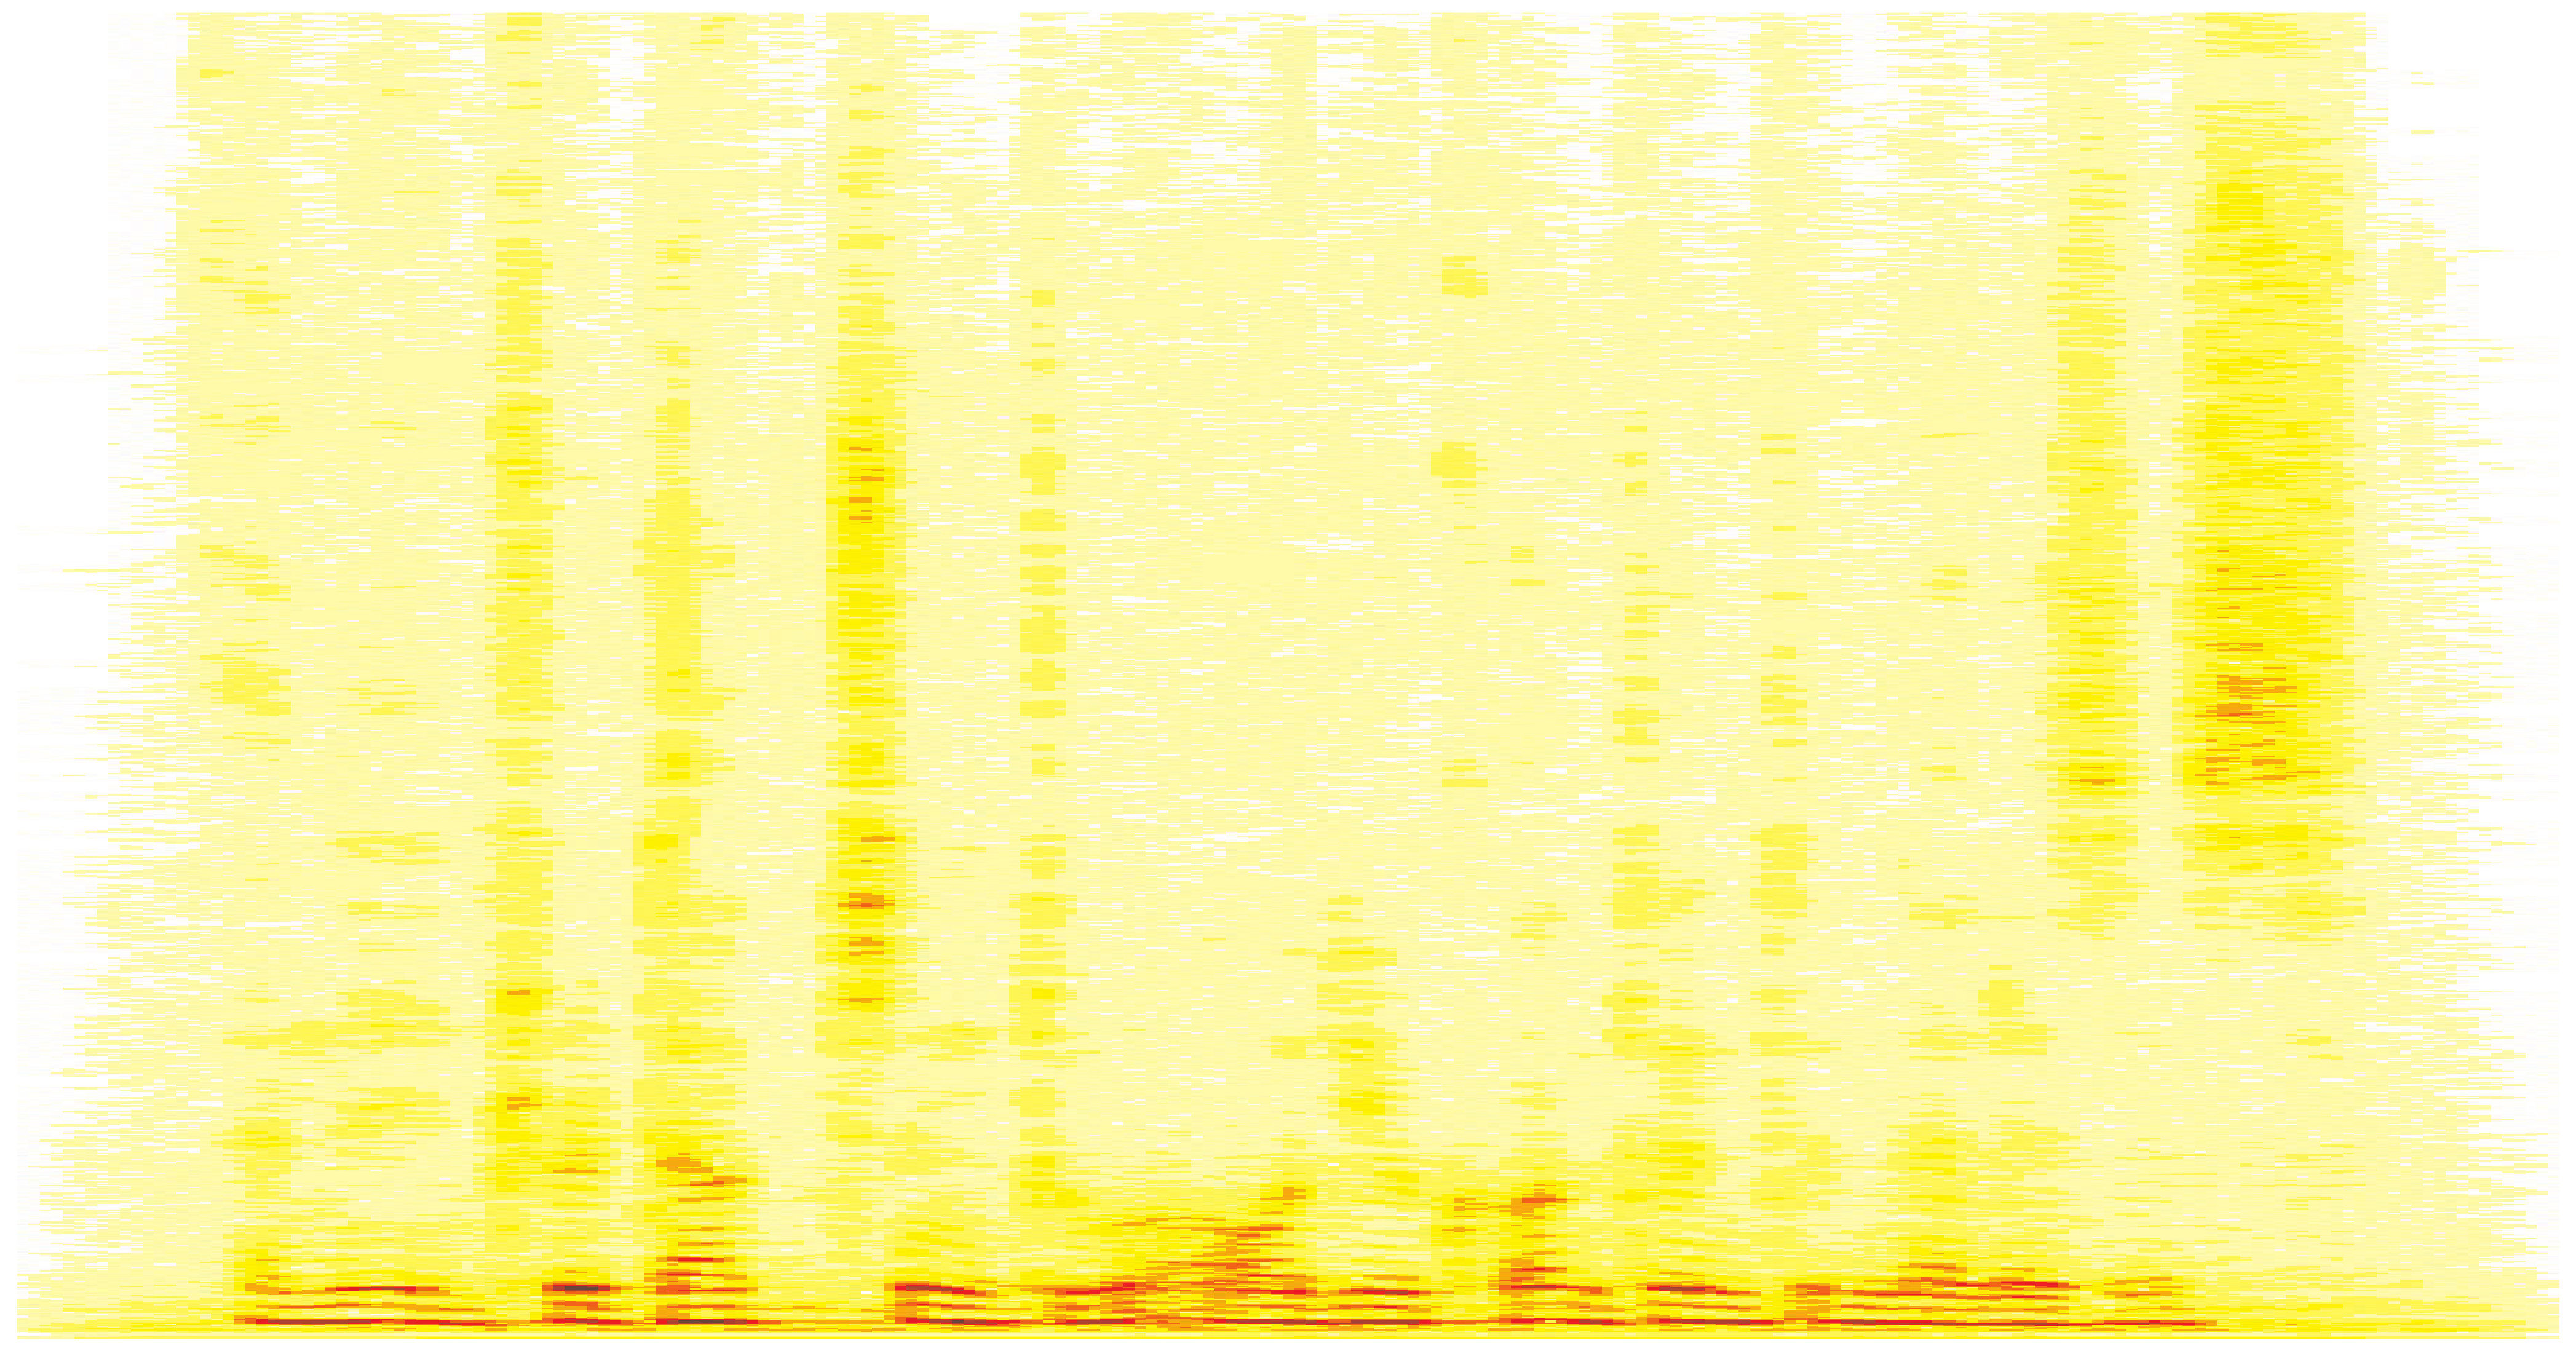
\includegraphics[width=\textwidth,height=3cm]{title}}

%%%%%%%%%%%%%%%%%%%%%%%%%%%%%%%%%%%%%%%%%%%%%%%%%%%%%%%%%%%%%%%%%%%%%%%%%%%%%%%%%%
%%%%%%%%%%%%%%%%%%%%%%%%%%%%%%%%%%%%%%%%%%%%%%%%%%%%%%%%%%%%%%%%%%%%%%%%%%%%%%%%%%
% colors
\definecolor{gtgold}{HTML}{E0AA0F} %{rgb}{0.88,0.66,1,0.06} [234, 170, 0]/256

%%%%%%%%%%%%%%%%%%%%%%%%%%%%%%%%%%%%%%%%%%%%%%%%%%%%%%%%%%%%%%%%%%%%%%%%%%%%%%%%%%
%%%%%%%%%%%%%%%%%%%%%%%%%%%%%%%%%%%%%%%%%%%%%%%%%%%%%%%%%%%%%%%%%%%%%%%%%%%%%%%%%%
% math
\DeclareMathOperator*{\argmax}{argmax}
\DeclareMathOperator*{\argmin}{argmin}
\DeclareMathOperator*{\atan}{atan}
\DeclareMathOperator*{\arcsinh}{arcsinh}
\DeclareMathOperator*{\sign}{sign}
\DeclareMathOperator*{\tcdf}{tcdf}
\DeclareMathOperator*{\si}{sinc}
\DeclareMathOperator*{\princarg}{princarg}
\DeclareMathOperator*{\arccosh}{arccosh}
\DeclareMathOperator*{\hwr}{HWR}
\DeclareMathOperator*{\flip}{flip}
\DeclareMathOperator*{\sinc}{sinc}
\DeclareMathOperator*{\floor}{floor}
\newcommand{\e}{{e}}
\newcommand{\jom}{\mathrm{j}\omega}
\newcommand{\jOm}{\mathrm{j}\Omega}
\newcommand   {\mat}[1]    		{\boldsymbol{\uppercase{#1}}}		%bold
\renewcommand {\vec}[1]    		{\boldsymbol{\lowercase{#1}}}		%bold

%%%%%%%%%%%%%%%%%%%%%%%%%%%%%%%%%%%%%%%%%%%%%%%%%%%%%%%%%%%%%%%%%%%%%%%%%%%%%%%%%%
%%%%%%%%%%%%%%%%%%%%%%%%%%%%%%%%%%%%%%%%%%%%%%%%%%%%%%%%%%%%%%%%%%%%%%%%%%%%%%%%%%
% media9
\newcommand{\includeaudio}[1]{{\includemedia[
                        addresource=audio/#1.mp3,
                        width=5mm,
                        height=5mm,
                        activate=onclick,
                        flashvars={
                            source=audio/#1.mp3  
                            &autoPlay=true
                        }]
                        {
\includegraphics[width=5mm, height=5mm]{SpeakerIcon}}
                        {APlayer.swf}}}
\newcommand{\audioautoplay}[1]{{\begin{center}\includemedia[
                            addresource=audio/#1.mp3,
                            width=.1\linewidth,
                            height=.01\linewidth,
                            activate=pageopen,
                            flashvars={
                                source=audio/#1.mp3  
                                &autoPlay=true
                            }]
                            {}
                            {APlayer.swf}\end{center}}}

\newcommand{\includevideo}[1]{{\begin{center}\includemedia[
                        addresource=video/#1.mp4,
                        width=0.8\linewidth,
                        height=0.4\linewidth,
                        activate=onclick,
                        flashvars={
                            source=video/#1.mp4  
                            &autoPlay=true
                        }]
                        {}
                        {VPlayer.swf}\end{center}}}
\newcommand{\videowithmatlab}[1]{{\begin{center}\includemedia[
                        addresource=video/animate#1.mp4,
                        width=0.8\linewidth,
                        height=0.4\linewidth,
                        activate=onclick,
                        flashvars={
                            source=video/animate#1.mp4  
                            &autoPlay=true
                        }]
                        {}
                        {VPlayer.swf}\end{center}\addreference{matlab source: matlab/animate#1.m}}}
                        

%%%%%%%%%%%%%%%%%%%%%%%%%%%%%%%%%%%%%%%%%%%%%%%%%%%%%%%%%%%%%%%%%%%%%%%%%%%%%%%%%%
%%%%%%%%%%%%%%%%%%%%%%%%%%%%%%%%%%%%%%%%%%%%%%%%%%%%%%%%%%%%%%%%%%%%%%%%%%%%%%%%%%
% other commands
\newcommand{\question}[1]{%\vspace{-4mm}
                          \setbeamercovered{invisible}
                          \begin{columns}[T]
                            \column{.8\textwidth}
                                \textbf{#1}
                            \column{.2\textwidth}
                                \vspace{-8mm}
                                \begin{flushright}
                                     
\includegraphics[scale=.5]{question_mark}
                                \end{flushright}
                                \vspace{6mm}
                          \end{columns}\pause\vspace{-12mm}}

\newcommand{\toremember}[1]{%\vspace{-4mm}
                          \begin{columns}[T]
                            \column{.8\textwidth}
                                \textbf{#1}
                            \column{.2\textwidth}
                                \vspace{-4mm}
                                \begin{flushright}
                                     
\includegraphics[scale=.5]{exclamation_mark}
                                \end{flushright}
                                \vspace{6mm}
                          \end{columns}\vspace{-6mm}}

\newcommand{\matlabexercise}[1]{%\vspace{-4mm}
                          \setbeamercovered{invisible}
                          \begin{columns}[T]
                            \column{.8\textwidth}
                                \textbf{matlab exercise}: #1
                            \column{.2\textwidth}
                                \begin{flushright}
                                     
\includegraphics[scale=.5]{logo_matlab}
                                \end{flushright}
                                %\vspace{6mm}
                          \end{columns}}

\newcommand{\addreference}[1]{  
                  
                    \begin{textblock*}{\baselineskip }(1.12\textwidth,.3\textheight) %(1.15\textwidth,.4\textheight)
                        \rotatebox{90}{\tiny {#1}}
                    \end{textblock*}}
                    
\newcommand{\figwithmatlab}[1]{
                    \begin{figure}
                        \centering
                        \includegraphics{#1}
                        %\label{fig:#1}
                    \end{figure}
                    
                    \addreference{matlab source: \href{https://github.com/alexanderlerch/ACA-Slides/blob/master/matlab/display#1.m}{matlab/display#1.m}}}
\newcommand{\figwithref}[2]{
                    \begin{figure}
                        \centering
                        \includegraphics{#1}
                        \label{fig:#1}
                    \end{figure}
                    
                    \addreference{#2}}  
                                    
\newcommand{\inserticon}[1]{

                    \begin{textblock*}{100mm}(14.5cm,7.5cm)
                        \includegraphics[height=.8cm,keepaspectratio]{#1}
                    \end{textblock*}}            

%%%%%%%%%%%%%%%%%%%%%%%%%%%%%%%%%%%%%%%%%%%%%%%%%%%%%%%%%%%%%%%%%%%%%%%%%%%%%%%%%%
%%%%%%%%%%%%%%%%%%%%%%%%%%%%%%%%%%%%%%%%%%%%%%%%%%%%%%%%%%%%%%%%%%%%%%%%%%%%%%%%%%
% counters
\newcounter{i}
\newcounter{j}
\newcounter{iXOffset}
\newcounter{iYOffset}
\newcounter{iXBlockSize}
\newcounter{iYBlockSize}
\newcounter{iYBlockSizeDiv2}
\newcounter{iDistance}



\subtitle{Module 1.0: Introduction to MIR/ACA}

%%%%%%%%%%%%%%%%%%%%%%%%%%%%%%%%%%%%%%%%%%%%%%%%%%%%%%%%%%%%%%%%%%%%%%%%%%%%
\begin{document}
    % generate title page
	

\begin{frame}
    \titlepage
    %\vspace{-5mm}
    \begin{flushright}
        \href{http://www.gtcmt.gatech.edu}{\includegraphics[height=.8cm,keepaspectratio]{logo_GTCMT_black}}
    \end{flushright}
\end{frame}


    \section[overview]{lecture overview}
        \begin{frame}{introduction}{overview}
            \begin{block}{corresponding textbook section}
                    \href{http://ieeexplore.ieee.org/xpl/articleDetails.jsp?tp=&arnumber=6331118&}{Chapter 1~---~Introduction}: pp.~1--6
            \end{block}

            \begin{itemize}
                \item   \textbf{lecture content}
                    \begin{itemize}
                        \item   audio content analysis
                        \item   typical applications
                        \item   audio content
                        \item   processing steps in a typical ACA system
                    \end{itemize}
                \bigskip
                \item<2->   \textbf{learning outcomes}
                    \begin{itemize}
                        \item   understand goals and applications in ACA
                        \item   know the typical forms of content in an audio signal
                        \item   understand the typical signal flow in an ACA system
                    \end{itemize}
            \end{itemize}
            \begin{textblock*}{100mm}(14.5cm,7.5cm)
                
\includegraphics[height=.8cm,keepaspectratio]{directions}
            \end{textblock*}
        \end{frame}
        
    \section[intro]{introduction}
        \begin{frame}{introduction}{audio content analysis --- terminology}
            \begin{itemize}
                \item   \textbf{goal}
                    \begin{itemize}
                        \item   extract information about the content of audio data
                    \end{itemize}
                \bigskip
                \item<2->   \textbf{terminology}
                    \begin{itemize}
                        \item	\textit{music information retrieval (MIR)}:
                            \begin{itemize}
                                \item   analysis and retrieval of music data 
                                \item   both audio and symbolic data
                            \end{itemize}
                                
                        \item	machine listening \& computer audition
                            \begin{itemize}
                                \item   focus on the recognition and understanding of music
                            \end{itemize}
                        \item	computational auditory scene analysis (CASA)
                            \begin{itemize}
                                \item   focus on human perception \& cognition, understanding of the auditory scene
                            \end{itemize}
                    \end{itemize}
           \end{itemize}
        \end{frame}
        \begin{frame}{introduction}{audio content analysis --- research field}
            \vspace{-7mm}
            \begin{columns}
            \column{.8\textwidth}
            \begin{itemize}
                \item<1->   \textbf{interdisciplinary}
                    \begin{itemize}
                        \item   digital signal processing
                        \item   machine learning / data mining
                        \item   musicology
                        \item   psycho-acoustics
                        \item   \ldots
                    \end{itemize}
                \smallskip
                \item<2->   ISMIR \textbf{community}
                            \begin{itemize}
                                \item   annual conferences
                                \item   conference papers \& Transactions
                                \item   ISMIR-Community mailing list
                                \item   MIREX: MIR Evaluation eXchange
                            \end{itemize}
                \smallskip
                \item<3->   \textbf{related publications} 
                    \begin{itemize}
                        \item   \textit{conferences}: ICASSP, ICME, SMC, DAFx, ACM~MM, \ldots
                        \item   \textit{journals}: TISMIR, TASLP, Computer Music, JNMR, JAES, \ldots
                    \end{itemize}
            \end{itemize}
            \column{.2\textwidth}
                \vspace{25mm}
                \begin{figure}
                    
\includegraphics[height=.8cm,keepaspectratio]{logo_ismir}
                \end{figure}
            \end{columns}
            \addreference{\href{http://www.ismir.net}{www.ismir.net}}
        \end{frame}
        \begin{frame}{introduction}{applications}
            \begin{itemize}
                \item	\textbf{organization} in large databases
                    \begin{itemize}
                        \item   search \& retrieval, classification, similarity
                    \end{itemize}
                \smallskip
                \item<2->	\textbf{interfaces} to search and retrieval
                    \begin{itemize}
                        \item   fingerprinting, query-by-humming systems
                    \end{itemize}
                \smallskip
                \item<3->	music \textbf{visualization}
                    \begin{itemize}
                        \item   symbolic (bars, harmony, score, \ldots), similarity mappings
                    \end{itemize}
                \smallskip
                \item<4->	adaptive \textbf{processing}
                    \begin{itemize}
                        \item   adaptive effect parametrization or algorithm selection
                    \end{itemize}
                \smallskip
                \item<5->	adaptive \textbf{interaction}
                    \begin{itemize}
                        \item   playlist generation, recommendation
                    \end{itemize}
            \end{itemize}
        \end{frame}
        \begin{frame}{introduction}{(commercial) examples}
            \setbeamercovered{invisible} % uncover the graphics with the bullet points
            \begin{itemize}
                \item   \textbf{recommendation}, playlist generation
                    \begin{columns}
                        \column{.25\textwidth}
                        \column{.25\textwidth}
                            
\includegraphics[scale=.1]{logo_spotify}
                        \column{.25\textwidth}
                            
\includegraphics[scale=.05]{logo_lastfm}
                        \column{.25\textwidth}
                            
\includegraphics[scale=.03]{logo_pandora}
                    \end{columns}
                \bigskip
                \item<2->   \textbf{fingerprinting} 
                    \begin{columns}
                        \column{.25\textwidth}
                        \column{.25\textwidth}
                            
\includegraphics[scale=.03]{logo_shazam}
                        \column{.25\textwidth}
                            
\includegraphics[scale=.05]{logo_gracenote}
                        \column{.25\textwidth}
                    \end{columns}
                \bigskip
                \item<3->   \textbf{score following} 
                   \begin{columns}
                        \column{.25\textwidth}
                        \column{.25\textwidth}
                            
\includegraphics[scale=.15]{logo_rockprodigy}
                        \column{.25\textwidth}
                            
\includegraphics[scale=.75]{logo_smartmusic}
                        \column{.25\textwidth}
                    \end{columns}
                \bigskip
                \item<4->   (multi-) \textbf{pitch detection} 
                    \begin{columns}
                        \column{.25\textwidth}
                        \column{.25\textwidth}
                            
\includegraphics[scale=.15]{logo_melodyne}
                        \column{.25\textwidth}
                        \column{.25\textwidth}
                    \end{columns}
            \end{itemize}
        \end{frame}

    \section[content]{audio content}
        \begin{frame}{audio content}{sources}
            \setbeamercovered{invisible}
            \question{what are the sources of (musical) audio content?}

            \begin{enumerate}
                \item<2->	\textbf{score}:
                    \begin{itemize}
                        \item   definition of musical ideas
                        \item   ``blue-print'' of the music
                        \item   \textit{examples}: melody, key, harmony, rhythmic patterns, \ldots
                    \end{itemize}
                \item<3->	\textbf{performance}:
                    \begin{itemize}
                        \item   unique acoustic rendition
                        \item   information in the score is interpreted, modified, added to
                        \item   \textit{examples}: (micro-)tempo, dynamics, intonation, \ldots
                    \end{itemize}
                \item<4->	\textbf{production}:
                    \begin{itemize}
                        \item   aesthetic choices 
                        \item   editing \& processing
                        \item   \textit{examples}: sound quality (EQ, microphone positioning), changes in timing and pitch
                    \end{itemize}
            \end{enumerate}
        \end{frame}
        \begin{frame}\frametitle{audio content}\framesubtitle{technical categories}
            audio content can be structured into \textbf{5 technical fundamental categories:}
            
            \bigskip
            \begin{enumerate}
                \item<2->	\textbf{timbral}: related to sound quality
                    \begin{itemize}
                        \item   \textit{examples}: instrument(ation), playing technique, venue, audio processing, \ldots
                    \end{itemize}
                \item<3->	\textbf{intensity-related}: related to musical dynamics
                    \begin{itemize}
                        \item   \textit{examples}: accents, loudness, \ldots
                    \end{itemize}
                \item<4->	\textbf{tonal}: related to pitch
                    \begin{itemize}
                        \item   \textit{examples}: melody, chords, intonation, vibrato, \ldots
                    \end{itemize}
                \item<5->	\textbf{temporal}: related to rhythm and tempo
                    \begin{itemize}
                        \item   \textit{examples}: timing, meter, rhythmic patterns, \ldots
                    \end{itemize}
                \item<6->	\textbf{statistical \& technical}: related to signal properties
                    \begin{itemize}
                        \item   \textit{examples}: amplitude distribution, number of zero crossings, \ldots
                    \end{itemize}
            \end{enumerate}
        \end{frame}

    \section[ACA]{generic audio content analysis system}
        \begin{frame}\frametitle{audio content analysis}\framesubtitle{system overview}
            \begin{figure}
                \centering
                \only<1>{\begin{footnotesize}
				\begin{picture}(96,26)
					\setcounter{iXOffset}{0}
					\setcounter{iYOffset}{5}
					\setcounter{iXBlockSize}{28}
					\setcounter{iYBlockSize}{16}
					\setcounter{iYBlockSizeDiv2}{8}
					\setcounter{iDistance}{8}
	
					\addtocounter{iYOffset}{\value{iYBlockSizeDiv2}}
					\addtocounter{iYOffset}{-2}
	
					%\addtocounter{iXOffset}{-1}
					\put(\value{iXOffset}, \value{iYOffset})
						{\text{{\shortstack[c]{audio\\ signal}}}}
					\addtocounter{iXOffset}{1}
	
					\addtocounter{iYOffset}{2}
					\addtocounter{iXOffset}{\value{iDistance}}
	
					\put(\value{iXOffset}, \value{iYOffset})
						{\vector(1,0){\value{iDistance}}}
	
					\addtocounter{iXOffset}{\value{iDistance}}
					\addtocounter{iYOffset}{-\value{iYBlockSizeDiv2}}
					
					\put(\value{iXOffset}, \value{iYOffset})
						{\framebox(\value{iXBlockSize}, \value{iYBlockSize}) {\color<2>{gtgold}{\shortstack[c]{feature\\ extraction}}}}
	
					\addtocounter{iXOffset}{\value{iXBlockSize}}
					\addtocounter{iYOffset}{\value{iYBlockSizeDiv2}}
	
					\put(\value{iXOffset}, \value{iYOffset})
						{\vector(1,0){\value{iDistance}}}
	
					\addtocounter{iXOffset}{\value{iDistance}}
					\addtocounter{iYOffset}{-\value{iYBlockSizeDiv2}}
	
					\put(\value{iXOffset}, \value{iYOffset})
						{\framebox(\value{iXBlockSize}, \value{iYBlockSize}) {\color<3>{gtgold}{\shortstack[c]{decision,\\ interpretation,\\ classification,\\ inference}}}}
	
					\addtocounter{iXOffset}{\value{iXBlockSize}}
					\addtocounter{iYOffset}{\value{iYBlockSizeDiv2}}
	
					\put(\value{iXOffset}, \value{iYOffset})
						{\vector(1,0){\value{iDistance}}}
	
					\addtocounter{iXOffset}{\value{iDistance}}
					\addtocounter{iYOffset}{-2}
	
					\addtocounter{iXOffset}{1}
					\put(\value{iXOffset}, \value{iYOffset})
						{\text{{\shortstack[c]{meta\\ data}}}}
					
				\end{picture}
\end{footnotesize}
}
                \only<2>{\begin{footnotesize}
				\begin{picture}(96,26)
					\setcounter{iXOffset}{0}
					\setcounter{iYOffset}{5}
					\setcounter{iXBlockSize}{28}
					\setcounter{iYBlockSize}{16}
					\setcounter{iYBlockSizeDiv2}{8}
					\setcounter{iDistance}{8}
	
					\addtocounter{iYOffset}{\value{iYBlockSizeDiv2}}
					\addtocounter{iYOffset}{-2}
	
					%\addtocounter{iXOffset}{-1}
					\put(\value{iXOffset}, \value{iYOffset})
						{\text{{\shortstack[c]{audio\\ signal}}}}
					\addtocounter{iXOffset}{1}
	
					\addtocounter{iYOffset}{2}
					\addtocounter{iXOffset}{\value{iDistance}}
	
					\put(\value{iXOffset}, \value{iYOffset})
						{\vector(1,0){\value{iDistance}}}
	
					\addtocounter{iXOffset}{\value{iDistance}}
					\addtocounter{iYOffset}{-\value{iYBlockSizeDiv2}}
					
					\put(\value{iXOffset}, \value{iYOffset})
						{\framebox(\value{iXBlockSize}, \value{iYBlockSize}) {\color{gtgold}{\shortstack[c]{feature\\ extraction}}}}
	
					\addtocounter{iXOffset}{\value{iXBlockSize}}
					\addtocounter{iYOffset}{\value{iYBlockSizeDiv2}}
	
					\put(\value{iXOffset}, \value{iYOffset})
						{\vector(1,0){\value{iDistance}}}
	
					\addtocounter{iXOffset}{\value{iDistance}}
					\addtocounter{iYOffset}{-\value{iYBlockSizeDiv2}}
	
					\put(\value{iXOffset}, \value{iYOffset})
						{\framebox(\value{iXBlockSize}, \value{iYBlockSize}) {\shortstack[c]{decision,\\ interpretation,\\ classification,\\ inference}}}
	
					\addtocounter{iXOffset}{\value{iXBlockSize}}
					\addtocounter{iYOffset}{\value{iYBlockSizeDiv2}}
	
					\put(\value{iXOffset}, \value{iYOffset})
						{\vector(1,0){\value{iDistance}}}
	
					\addtocounter{iXOffset}{\value{iDistance}}
					\addtocounter{iYOffset}{-2}
	
					\addtocounter{iXOffset}{1}
					\put(\value{iXOffset}, \value{iYOffset})
						{\text{{\shortstack[c]{meta\\ data}}}}
					
				\end{picture}
\end{footnotesize}
}
                \only<3->{\begin{footnotesize}
				\begin{picture}(96,26)
					\setcounter{iXOffset}{0}
					\setcounter{iYOffset}{5}
					\setcounter{iXBlockSize}{28}
					\setcounter{iYBlockSize}{16}
					\setcounter{iYBlockSizeDiv2}{8}
					\setcounter{iDistance}{8}
	
					\addtocounter{iYOffset}{\value{iYBlockSizeDiv2}}
					\addtocounter{iYOffset}{-2}
	
					%\addtocounter{iXOffset}{-1}
					\put(\value{iXOffset}, \value{iYOffset})
						{\text{{\shortstack[c]{audio\\ signal}}}}
					\addtocounter{iXOffset}{1}
	
					\addtocounter{iYOffset}{2}
					\addtocounter{iXOffset}{\value{iDistance}}
	
					\put(\value{iXOffset}, \value{iYOffset})
						{\vector(1,0){\value{iDistance}}}
	
					\addtocounter{iXOffset}{\value{iDistance}}
					\addtocounter{iYOffset}{-\value{iYBlockSizeDiv2}}
					
					\put(\value{iXOffset}, \value{iYOffset})
						{\framebox(\value{iXBlockSize}, \value{iYBlockSize}) {\shortstack[c]{feature\\ extraction}}}
	
					\addtocounter{iXOffset}{\value{iXBlockSize}}
					\addtocounter{iYOffset}{\value{iYBlockSizeDiv2}}
	
					\put(\value{iXOffset}, \value{iYOffset})
						{\vector(1,0){\value{iDistance}}}
	
					\addtocounter{iXOffset}{\value{iDistance}}
					\addtocounter{iYOffset}{-\value{iYBlockSizeDiv2}}
	
					\put(\value{iXOffset}, \value{iYOffset})
						{\framebox(\value{iXBlockSize}, \value{iYBlockSize}) {\color{gtgold}{\shortstack[c]{decision,\\ interpretation,\\ classification,\\ inference}}}}
	
					\addtocounter{iXOffset}{\value{iXBlockSize}}
					\addtocounter{iYOffset}{\value{iYBlockSizeDiv2}}
	
					\put(\value{iXOffset}, \value{iYOffset})
						{\vector(1,0){\value{iDistance}}}
	
					\addtocounter{iXOffset}{\value{iDistance}}
					\addtocounter{iYOffset}{-2}
	
					\addtocounter{iXOffset}{1}
					\put(\value{iXOffset}, \value{iYOffset})
						{\text{{\shortstack[c]{meta\\ data}}}}
					
				\end{picture}
\end{footnotesize}
}
            \end{figure}
            
            \begin{columns}
                \column{.5\textwidth}
                    \begin{itemize}
                        \item<2->[]	\textbf{feature extraction}
                                \begin{itemize}
                                    \item 	dimensionality reduction
                                    \item	meaningful representation
                                \end{itemize}
                    \end{itemize}
                \column{.5\textwidth}
                    \begin{itemize}
                        \item<3->[]	\textbf{classification}
                                \begin{itemize}
                                    \item	map or convert feature to comprehensible domain
                                \end{itemize}
                    \end{itemize}
            \end{columns}
        \end{frame}

    \section{summary}
        \begin{frame}{summary}{lecture content}
            \begin{itemize}
                \item       what is audio content?
                \bigskip
                \item<2->   what are the technical categories of interest?
                \bigskip
                \item<3->   what are the typical processing blocks of an ACA system?
            \end{itemize}
            \begin{textblock*}{100mm}(14.5cm,7.5cm)
                
\includegraphics[height=.8cm,keepaspectratio]{summary}
            \end{textblock*}
        \end{frame}
\end{document}
